\documentclass{article}

\usepackage{amsmath}
\usepackage{tikz}
\usepackage{pgfplots}
\pgfplotsset{compat=1.18}
\usepackage{xcolor}

\title{Midetrm 1 Study Guide}
\author{Mondai, Physics 122, Winter 2026, Cal Poly}


\begin{document}
\maketitle


\section*{ Efficiency}

\subsection*{Concept Summary}
Efficiency measures how much useful output energy (or work) you get compared to the energy input:
\[
e = \frac{E_{\text{useful}}}{E_{\text{input}}}
\]
Efficiency is often expressed as a percentage.

Common pitfalls:
\begin{itemize}
  \item Forgetting that efficiency is always less than 1 (or 100\%).
  \item Mixing up input and useful output energy.
\end{itemize}

\subsection*{Example Problem}
An engine takes in $500\,\text{J}$ of energy and produces $150\,\text{J}$ of useful work.
\begin{enumerate}
  \item What is the efficiency?
  \item How much energy is wasted?
\end{enumerate}

\subsection*{Solution}

\textcolor{blue}{
\textbf{Concept:} Efficiency compares useful output energy to total input energy.
}

\textcolor{blue}{
\textbf{Diagram:}  
[DIAGRAM PLACEHOLDER: Energy input arrow splitting into useful work and wasted energy]
}

\textcolor{blue}{
\textbf{Algebra:}
\[
e = \frac{E_{\text{useful}}}{E_{\text{input}}}
\]
}

\textcolor{blue}{
\textbf{Numbers:}
\[
e = \frac{150}{500} = 0.30 = 30\%
\]
\[
E_{\text{wasted}} = 500 - 150 = 350\,\text{J}
\]
}

\textcolor{blue}{
\textbf{Assess:}  
Efficiency is less than 100\%, which is realistic. Energy is conserved since useful plus wasted energy equals the input.
}

\section*{ Energy Use in the Human Body}

\subsection*{Concept Summary}
The human body converts chemical energy from food into useful work and thermal energy. Like all systems, the body is not 100\% efficient.

Common pitfalls:
\begin{itemize}
  \item Assuming all food energy becomes useful work.
  \item Forgetting that most energy becomes thermal energy.
\end{itemize}

\subsection*{Example Problem}
A cyclist uses $2000\,\text{J}$ of chemical energy while pedaling and produces $400\,\text{J}$ of mechanical work.
\begin{enumerate}
  \item What is the efficiency of the cyclist?
  \item How much energy becomes thermal energy?
\end{enumerate}

\subsection*{Solution}

\textcolor{blue}{
\textbf{Concept:} The body converts chemical energy into work, with the remainder becoming thermal energy.
}

\textcolor{blue}{
\textbf{Diagram:}  
[DIAGRAM PLACEHOLDER: Chemical energy in body converting to work and thermal energy]
}

\textcolor{blue}{
\textbf{Algebra:}
\[
e = \frac{W_{\text{out}}}{E_{\text{chem}}}
\]
}

\textcolor{blue}{
\textbf{Numbers:}
\[
e = \frac{400}{2000} = 0.20 = 20\%
\]
\[
E_{\text{thermal}} = 2000 - 400 = 1600\,\text{J}
\]
}

\textcolor{blue}{
\textbf{Assess:}  
A 20\% efficiency is reasonable for human muscles. Energy is conserved.
}

\section*{ The First Law of Thermodynamics}

\subsection*{Concept Summary}
The First Law of Thermodynamics relates changes in a system’s internal energy to energy transfers:
\[
\Delta E_{\text{int}} = Q + W_{env}
\]
where $Q$ is heat added to the system and $W$ is work done by the system.

Common pitfalls:
\begin{itemize}
  \item Using the wrong sign for work.
  \item Forgetting that work done \emph{by} the system is positive if the dispalcement and $F_{gas}$ are in the same direction. 
\end{itemize}

\subsection*{Example Problem}
A gas absorbs $300\,\text{J}$ of heat and does $100\,\text{J}$ of work on its surroundings.
\begin{enumerate}
  \item What is the change in internal energy of the gas?
\end{enumerate}

\subsection*{Solution}

\textcolor{blue}{
\textbf{Concept:} Internal energy changes based on heat added and work done by the system.
}

\textcolor{blue}{
\textbf{Diagram:}  
[DIAGRAM PLACEHOLDER: Gas in cylinder with heat entering and piston moving]
}

\textcolor{blue}{
\textbf{Algebra:}
\[
\Delta E_{\text{int}} = Q + W_{env}
\]
}

\textcolor{blue}{
\textbf{Numbers:}
\[
\Delta E_{\text{int}} = 300 - 100 = 200\,\text{J}
\]
}

\textcolor{blue}{
\textbf{Assess:}  
The internal energy increases, which makes sense because more heat was added than work done.
}


\section*{Example: Heat and Work from a PV Diagram}

\subsection*{Problem}
A gas undergoes the process shown on the $PV$ diagram below.  
The pressure remains constant at $P = 200\,\text{kPa}$ while the volume increases from
$V_1 = 1.0\,\text{m}^3$ to $V_2 = 3.0\,\text{m}^3$.

During this process, the internal energy of the gas increases by $200\,\text{J}$.

\begin{enumerate}
  \item What is the work done by the environment on the gas?
  \item How much heat is transferred to the gas?
\end{enumerate}

\subsection*{PV Diagram}

\begin{center}
\begin{tikzpicture}[scale=1.1]
  % Axes
  \draw[->] (0,0) -- (4.5,0) node[right] {$V$ (m$^3$)};
  \draw[->] (0,0) -- (0,3.5) node[above] {$P$ (kPa)};

  % Constant pressure line
  \draw[thick, blue] (1,2) -- (3,2);

  % Points
  \fill (1,2) circle (2pt) node[below] {$V_1$};
  \fill (3,2) circle (2pt) node[below] {$V_2$};

  % Labels
  \node[left] at (0,2) {$200$};
  \draw[dashed] (1,2) -- (1,0);
  \draw[dashed] (3,2) -- (3,0);

  % Arrow indicating process
  \draw[->, thick] (1.8,2.15) -- (2.2,2.15);
\end{tikzpicture}
\end{center}

\subsection*{Solution}

\textcolor{blue}{
\textbf{Concept:}  
On a $PV$ diagram, the work magnitude equals the area under the curve. For expansion, the environment does negative work on the gas. Heat is found using the First Law,
$\Delta E = Q + W_{\text{env}}$.
}

\textcolor{blue}{
\textbf{Algebra:}
\[
W_{\text{env}} = -P\,\Delta V
\]
\[
\Delta E = Q + W_{\text{env}}
\]
}

\textcolor{blue}{
\textbf{Numbers:}
\[
\Delta V = 3.0 - 1.0 = 2.0\,\text{m}^3
\]
\[
W_{\text{env}} = -(200\,\text{kPa})(2.0\,\text{m}^3)
= -(2.0\times10^5)(2.0)
= -4.0\times10^5\,\text{J}
\]
\[
Q = \Delta E - W_{\text{env}}
= 200 - (-4.0\times10^5)
= 4.002\times10^5\,\text{J}
\]
}

\textcolor{blue}{
\textbf{Assess:}  
The negative work confirms expansion. Most of the added heat goes into work done on the surroundings, which is consistent with the large area under the curve.
}


\section*{Example: Entropy (Conceptual)}

\subsection*{Concept Summary}
Entropy is a measure of how energy is spread out or how many microscopic arrangements (microstates) are possible. Natural processes tend to move toward higher entropy.

% Common pitfalls:
% \begin{itemize}
%   \item Thinking entropy means ``disorder'' instead of energy spreading.
%   \item Assuming entropy must increase everywhere rather than for the universe as a whole.
% \end{itemize}

\subsection*{Example Problem}
A hot metal block is placed in contact with a cold metal block inside an insulated box.
Energy flows from the hot block to the cold block until they reach the same temperature.

\begin{enumerate}
  \item Does the entropy of the hot block increase or decrease?
  \item Does the entropy of the cold block increase or decrease?
  \item Does the total entropy of the two-block system increase, decrease, or stay the same?
\end{enumerate}

\subsection*{Solution}

\textcolor{blue}{
\textbf{Concept:}  
Entropy increases when energy spreads out. Heat flowing from hot to cold increases the number of accessible microstates.
}

\textcolor{blue}{
\textbf{Diagram:}  
[DIAGRAM PLACEHOLDER: Hot block and cold block with heat flowing from hot to cold]
}

\textcolor{blue}{
\textbf{Reasoning:}
\begin{itemize}
  \item The hot block loses energy, so its entropy decreases.
  \item The cold block gains energy, so its entropy increases.
  \item The increase in entropy of the cold block is greater than the decrease in entropy of the hot block.
\end{itemize}
}

\textcolor{blue}{
\textbf{Conclusion:}  
The total entropy of the two-block system increases, which is why heat flows spontaneously from hot to cold.
}

\textcolor{blue}{
\textbf{Assess:}  
This process is irreversible and consistent with the Second Law of Thermodynamics: entropy of an isolated system increases.
}

\section*{Chapter 12: Temperature and Heat}

\section*{Temperature, Thermal Energy, and Molecular Speed}

\subsection*{Concept Summary}
\begin{itemize}
  \item \textbf{Temperature} measures the \emph{average kinetic energy} of the particles in a substance.
  \item \textbf{Thermal energy} is the \emph{total} kinetic energy of all particles and depends on both temperature and the amount of substance.
  \item The \textbf{root-mean-square speed} $v_{\text{rms}}$ describes the typical speed of particles in a gas and depends only on temperature and particle mass.
\end{itemize}

Key ideas:
\begin{itemize}
  \item Higher temperature $\Rightarrow$ faster average particle motion.
  \item Larger objects can have more thermal energy even at the same temperature.
  \item At the same temperature, lighter molecules move faster than heavier ones.
\end{itemize}

Common pitfalls:
\begin{itemize}
  \item Confusing temperature with thermal energy.
  \item Thinking individual particles all move at the same speed.
  \item Assuming heavier molecules move faster at the same temperature.
\end{itemize}

\subsection*{Example Problem}
Two sealed containers, A and B, hold ideal gases at the same temperature.
Container A holds helium atoms, while container B holds oxygen molecules.

\begin{enumerate}
  \item Which container has gas particles with the greater average kinetic energy?
  \item Which gas has the greater $v_{\text{rms}}$?
  \item If container B has more gas particles than container A, which container has more thermal energy?
\end{enumerate}

\subsection*{Solution}

\textcolor{blue}{
\textbf{Concept:}  
Temperature determines average kinetic energy. Thermal energy depends on both temperature and the number of particles. The rms speed depends on temperature and particle mass.
}

\textcolor{blue}{
\textbf{Diagram:}  
[DIAGRAM PLACEHOLDER: Two containers at same temperature; light helium particles moving faster than heavier oxygen molecules]
}

\textcolor{blue}{
\textbf{Reasoning:}
\begin{itemize}
  \item Since the temperatures are the same, particles in both containers have the same average kinetic energy.
  \item Helium atoms are much lighter than oxygen molecules, so helium has the larger $v_{\text{rms}}$.
  \item Container B has more particles, so it has greater total thermal energy.
\end{itemize}
}

\textcolor{blue}{
\textbf{Assess:}  
These results are consistent with molecular theory: temperature sets average kinetic energy, mass affects speed, and thermal energy scales with the number of particles.
}

\section*{ The Ideal Gas Law}

\subsection*{Concept Summary}
An ideal gas is a simplified model in which gas particles:
\begin{itemize}
  \item Have negligible volume compared to the container.
  \item Do not exert forces on each other except during collisions.
\end{itemize}

For an ideal gas, pressure, volume, temperature, and the amount of gas are related by:
\[
PV = nRT
\]
where:
\begin{itemize}
  \item $P$ is pressure,
  \item $V$ is volume,
  \item $n$ is the number of moles,
  \item $R = 8.31\,\text{J/(mol·K)}$,
  \item $T$ is temperature in kelvins.
\end{itemize}

Key ideas:
\begin{itemize}
  \item Temperature must always be in kelvins.
  \item Increasing temperature increases molecular speed and pressure (if volume is fixed).
  \item The ideal gas law connects macroscopic quantities to microscopic motion.
\end{itemize}

Common pitfalls:
\begin{itemize}
  \item Using Celsius instead of kelvins.
  \item Forgetting that pressure depends on molecular collisions with container walls.
\end{itemize}

\subsection*{Example Problem}
A container holds $1.0\,\text{mol}$ of an ideal gas at a temperature of $300\,\text{K}$.
The gas occupies a volume of $0.25\,\text{m}^3$.

\begin{enumerate}
  \item What is the pressure of the gas?
  \item If the temperature increases while volume stays constant, what happens to the pressure?
\end{enumerate}

\subsection*{Solution}

\textcolor{blue}{
\textbf{Concept:}  
The ideal gas law relates pressure to temperature, volume, and the number of moles. At fixed volume, pressure is directly proportional to temperature.
}

\textcolor{blue}{
\textbf{Diagram:}  
[DIAGRAM PLACEHOLDER: Gas particles colliding with the walls of a rigid container]
}

\textcolor{blue}{
\textbf{Algebra:}
\[
P = \frac{nRT}{V}
\]
}

\textcolor{blue}{
\textbf{Numbers:}
\[
P = \frac{(1.0)(8.31)(300)}{0.25}
\]
\[
P = \frac{2493}{0.25} \approx 1.0\times10^4\,\text{Pa}
\]
}

\textcolor{blue}{
\textbf{Reasoning (Part 2):}  
If the temperature increases while the volume stays constant, gas particles move faster and collide more often with the walls, so the pressure increases.
}

\textcolor{blue}{
\textbf{Assess:}  
The pressure is reasonable for a low-density gas. The direct relationship between pressure and temperature is consistent with kinetic theory.
}


\subsection*{Constant-Pressure (Isobaric) Process}

\textbf{Example:} One mole of an ideal gas expands at constant pressure
$P = 2.0\times 10^{5}\ \mathrm{Pa}$. The volume increases from
$V_i = 0.010\ \mathrm{m}^3$ to $V_f = 0.030\ \mathrm{m}^3$.

\textcolor{blue}{
\textbf{Concept:} At constant pressure, the $PV$ path is a horizontal
line. The work done by the environment equals the negative of the area
under this line on a $PV$ diagram.
}

\begin{center}
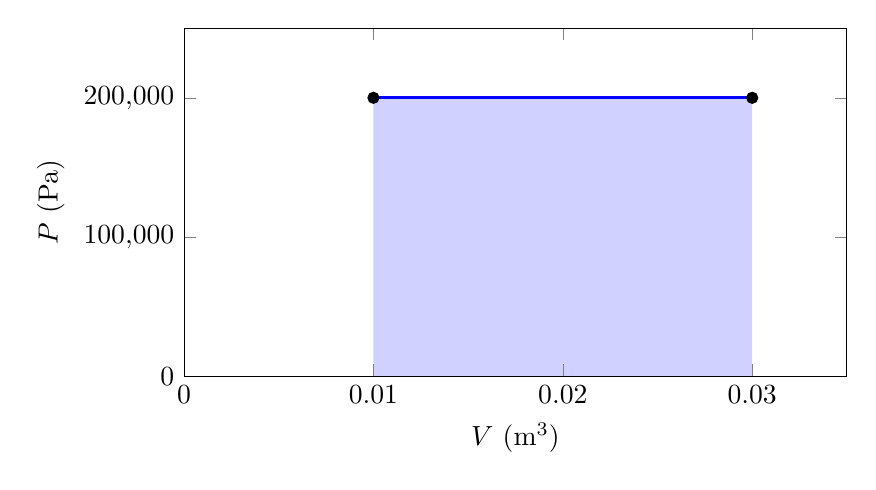
\begin{tikzpicture}
  \begin{axis}[
    width=10cm, height=6cm,
    xlabel={$V\ (\mathrm{m}^3)$},
    ylabel={$P\ (\mathrm{Pa})$},
    xmin=0, xmax=0.035,
    ymin=0, ymax=2.5e5,
    xtick={0.00,0.01,0.02,0.03},
    ytick={0,1e5,2e5},
    scaled ticks=false,
    ticklabel style={/pgf/number format/fixed},
    axis on top
  ]

  % isobaric line
  \addplot[blue, very thick] coordinates {(0.010,2e5) (0.030,2e5)};

  % shaded work area
  \addplot[fill=blue, fill opacity=0.18, draw=none] coordinates
    {(0.010,0) (0.010,2e5) (0.030,2e5) (0.030,0)} \closedcycle;

  % initial and final points
  \addplot[only marks, mark=*] coordinates {(0.010,2e5) (0.030,2e5)};

  \end{axis}
\end{tikzpicture}
\end{center}

\textcolor{blue}{
\textbf{Algebra:}
\[
W_{\text{env}} = -P\,\Delta V
\]
\textbf{Numbers:}
\[
\Delta V = 0.030 - 0.010 = 0.020\ \mathrm{m}^3
\]
\[
W_{\text{env}} = -(2.0\times10^{5})(0.020)
= -4.0\times10^{3}\ \mathrm{J}
\]
\textbf{Assess:} The negative sign is correct because the gas expands.
The magnitude is reasonable for this pressure and volume change.
}

\subsection*{Constant-Volume (Isochoric) Process}

\textbf{Example:} One mole of an ideal gas is heated at constant volume
$V = 0.020\ \mathrm{m}^3$. The pressure increases from
$P_i = 1.0\times10^{5}\ \mathrm{Pa}$ to
$P_f = 3.0\times10^{5}\ \mathrm{Pa}$.  
\textbf{Find the heat $Q$ added to the gas.}

\textcolor{blue}{
\textbf{Concept:} In a constant-volume process the $PV$ path is vertical,
so no work is done by or on the gas. Any change in internal energy must
come entirely from heat transfer.
}

\begin{center}
\begin{tikzpicture}
  \begin{axis}[
    width=10cm, height=6cm,
    xlabel={$V\ (\mathrm{m}^3)$},
    ylabel={$P\ (\mathrm{Pa})$},
    xmin=0, xmax=0.035,
    ymin=0, ymax=3.5e5,
    xtick={0.00,0.01,0.02,0.03},
    ytick={0,1e5,2e5,3e5},
    scaled ticks=false,
    ticklabel style={/pgf/number format/fixed},
    axis on top
  ]

  % isochoric vertical line
  \addplot[blue, very thick] coordinates {(0.020,1e5) (0.020,3e5)};

  % initial and final points
  \addplot[only marks, mark=*] coordinates {(0.020,1e5) (0.020,3e5)};

  \end{axis}
\end{tikzpicture}
\end{center}

\textcolor{blue}{
\textbf{Algebra:}
First Law of Thermodynamics:
\[
\Delta E = Q + W_{\text{env}}
\]
For a constant-volume process:
\[
W_{\text{env}} = 0
\]
For an ideal gas:
\[
\Delta E = \frac{3}{2}nR\Delta T
\]
\textbf{Numbers:}
Use the ideal gas law to find the temperature change:
\[
T = \frac{PV}{nR}
\]
\[
T_i = \frac{(1.0\times10^{5})(0.020)}{(1)(8.31)} \approx 240\ \mathrm{K}
\]
\[
T_f = \frac{(3.0\times10^{5})(0.020)}{(1)(8.31)} \approx 720\ \mathrm{K}
\]
\[
\Delta T = 720 - 240 = 480\ \mathrm{K}
\]
\[
\Delta E = \frac{3}{2}(1)(8.31)(480) \approx 6.0\times10^{3}\ \mathrm{J}
\]
Since $W_{\text{env}}=0$:
\[
Q = \Delta E \approx 6.0\times10^{3}\ \mathrm{J}
\]
\textbf{Assess:} The heat is positive, as expected for heating the gas.
The magnitude is reasonable for a large temperature increase at fixed
volume.
}


\subsection*{Constant-Temperature (Isothermal) Process}

\textbf{Example:} One mole of an ideal gas undergoes an isothermal
expansion at temperature $T = 300\ \mathrm{K}$. The volume increases from
$V_i = 0.010\ \mathrm{m}^3$ to $V_f = 0.040\ \mathrm{m}^3$.

\textcolor{blue}{\textbf{Concept:} In an isothermal process the temperature remains constant, so the gas obeys $PV=\text{constant}$. The $PV$ diagram is a downward-curving hyperbola, and the work done by the environment equals the signed area under this curve.}

\begin{center}
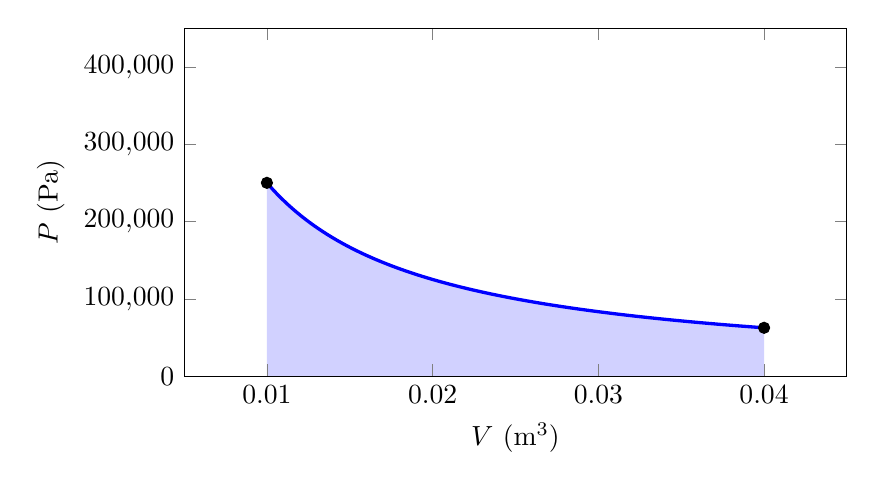
\begin{tikzpicture}
  \begin{axis}[
    width=10cm, height=6cm,
    xlabel={$V\ (\mathrm{m}^3)$},
    ylabel={$P\ (\mathrm{Pa})$},
    xmin=0.005, xmax=0.045,
    ymin=0, ymax=4.5e5,
    xtick={0.01,0.02,0.03,0.04},
    ytick={0,1e5,2e5,3e5,4e5},
    scaled ticks=false,
    ticklabel style={/pgf/number format/fixed},
    axis on top,
    domain=0.01:0.04,
    samples=100
  ]

  % isothermal curve: P = (nRT)/V
  \addplot[blue, very thick] {2500/x};

  % shaded work area
  \addplot[fill=blue, fill opacity=0.18, draw=none]
    ({x}, {2500/x}) \closedcycle;

  % initial and final points
  \addplot[only marks, mark=*] coordinates {(0.010,2.5e5) (0.040,6.25e4)};

  \end{axis}
\end{tikzpicture}
\end{center}

% \textcolor{blue}{\textbf{Algebra:} The work done by the environment for an isothermal ideal-gas process is $W_{\text{env}}=-nRT\ln\!\left(\frac{V_f}{V_i}\right)$.}

% \textcolor{blue}{\textbf{Numbers:} Substituting values gives $W_{\text{env}}=-(1)(8.31)(300)\ln(4)\approx -3.5\times10^{3}\ \mathrm{J}$.}

% \textcolor{blue}{\textbf{Assess:} The work is negative, consistent with an expanding gas, and the magnitude is reasonable for a fourfold increase in volume at room temperature.}


\subsection*{Adiabatic Process (Conceptual)}

\textbf{Example:} An ideal gas expands adiabatically inside an insulated
cylinder, so no heat enters or leaves the gas during the process.

\textcolor{blue}{\textbf{Concept:} In an adiabatic process there is no heat transfer ($Q=0$), so any work done by the gas comes at the expense of its internal energy. As the gas expands, its temperature decreases. On a $PV$ diagram, an adiabatic curve slopes downward more steeply than an isothermal curve passing through the same initial point.}

\begin{center}
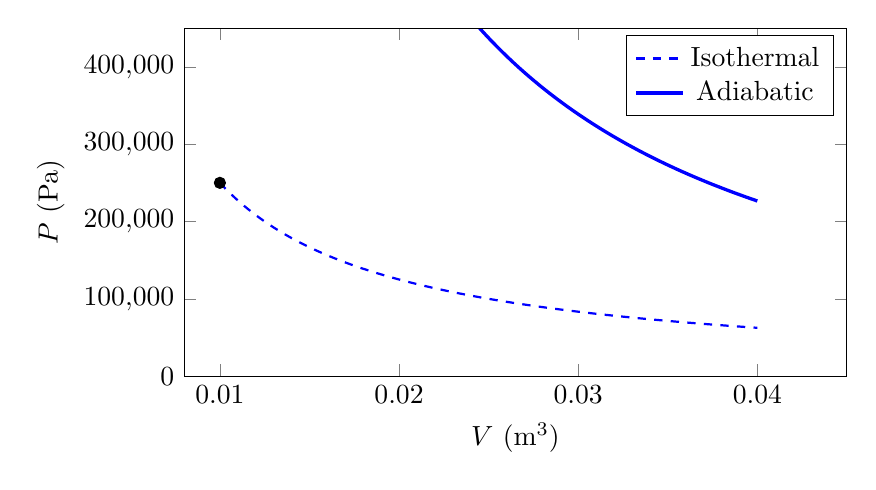
\begin{tikzpicture}
  \begin{axis}[
    width=10cm, height=6cm,
    xlabel={$V\ (\mathrm{m}^3)$},
    ylabel={$P\ (\mathrm{Pa})$},
    xmin=0.008, xmax=0.045,
    ymin=0, ymax=4.5e5,
    xtick={0.01,0.02,0.03,0.04},
    ytick={0,1e5,2e5,3e5,4e5},
    scaled ticks=false,
    ticklabel style={/pgf/number format/fixed},
    axis on top,
    domain=0.01:0.04,
    samples=100
  ]

  % isothermal curve (reference)
  \addplot[blue, thick, dashed] {2500/x};
  \addlegendentry{Isothermal}

  % adiabatic curve (steeper)
  \addplot[blue, very thick] {2500/x^(1.4)};
  \addlegendentry{Adiabatic}

  % initial point
  \addplot[only marks, mark=*] coordinates {(0.010,2.5e5)};

  \end{axis}
\end{tikzpicture}
\end{center}

\textcolor{blue}{\textbf{Assess:} The steeper adiabatic curve reflects the fact that pressure drops more rapidly with volume than in an isothermal process because the gas cools as it does work with no heat input.}


\subsection*{1D Thermal Expansion (Linear)}

\textbf{Example:} A steel rod has an initial length
$L_0 = 2.0\ \mathrm{m}$ at $20^\circ\mathrm{C}$.
The temperature increases to $120^\circ\mathrm{C}$.
The coefficient of linear expansion for steel is
$\alpha = 1.2\times10^{-5}\ \mathrm{^\circ C^{-1}}$.
Find the change in length of the rod.

\textcolor{blue}{\textbf{Concept:} In one-dimensional thermal expansion, the change in length is proportional to the original length and the temperature change.}

\textcolor{blue}{\textbf{Algebra:} The linear expansion formula is $\Delta L = \alpha L_0 \Delta T$.}

\textcolor{blue}{\textbf{Numbers:} The temperature change is $\Delta T = 120 - 20 = 100^\circ\mathrm{C}$. Substituting gives $\Delta L = (1.2\times10^{-5})(2.0)(100) = 2.4\times10^{-3}\ \mathrm{m}$.}

\textcolor{blue}{\textbf{Assess:} The rod length increases by $2.4\ \mathrm{mm}$, which is reasonable for steel over a $100^\circ\mathrm{C}$ temperature change.}


\subsection*{3D Thermal Expansion (Volume)}

\textbf{Example:} A solid aluminum block has an initial volume
$V_0 = 1.0\times10^{-2}\ \mathrm{m}^3$ at $20^\circ\mathrm{C}$.
The temperature increases to $70^\circ\mathrm{C}$.
The coefficient of linear expansion for aluminum is
$\alpha = 2.3\times10^{-5}\ \mathrm{^\circ C^{-1}}$.
Find the change in volume of the block.

\textcolor{blue}{\textbf{Concept:} In three dimensions the object expands independently along three perpendicular directions. For small temperature changes, the volume expansion coefficient is approximately $3\alpha$, extending the 2D result where the area expansion coefficient is $2\alpha$.}

\textcolor{blue}{\textbf{Algebra:} The volume expansion formula is $\Delta V = 3\alpha V_0 \Delta T$.}

\textcolor{blue}{\textbf{Numbers:} The temperature change is $\Delta T = 70 - 20 = 50^\circ\mathrm{C}$. Substituting gives $\Delta V = 3(2.3\times10^{-5})(1.0\times10^{-2})(50) = 3.45\times10^{-5}\ \mathrm{m}^3$.}

\textcolor{blue}{\textbf{Assess:} The volume increase is much smaller than the original volume, consistent with the assumption of small thermal expansion and validating the linear approximation.}

\end{document}
